\section{Modelos de Consistência}

\subsection{Motivação}

\begin{frame}{Content Delivery Network}
\includegraphics[width=.7\textwidth]{images/cdn}

\begin{itemize}
	\item Conteúdo é colocado próximo aos clientes. 
	\item Conteúdo estático ou majoritariamente determinístico. 
	\item Um pequeno atraso na replicação é tolerado.
	\item Atualização acontece infrequentemente.
\end{itemize}

Fonte: \url{https://www.creative-artworks.eu/why-use-a-content-delivery-network-cdn/}
\end{frame}


\begin{frame} {RAFT}
Considere um sistema replicado usando RAFT. Após cada operação que modifica o estado, todas as réplicas tem o mesmo valor.

\includegraphics[width=.5\textwidth]{images/raft} %Fonte: http://thesecretlivesofdata.com/raft/

Caso um cliente queira apenas ler o estado, o que deve fazer?
\pause
\begin{itemize}
	\item Requisitar o valor do líder\pause : o valor lido será \alert{o último} valor escrito.\pause
	\item Requisitar o valor de alguma réplica\pause : o valor lido será \alert{um} valor escrito, não necessariamente o último. Mais tempo implica maior a probabilidade de ser o valor escrito.\pause
	\item Se em vez de difusão atômica usássemos IP-Multicast?\pause{} Alguns valores escritos poderiam nunca ser vistos.
\end{itemize}
\end{frame}

\begin{frame}{Replicação: solução ou problema?}
	Replicação aumenta disponibilidade mas tem custo em desempenho e, possivelmente, inconsistências temporárias nos dados.
\end{frame}

\begin{frame}{Conflitos}
O problema da replicação está em como lidar com conflitos nas operações dos clientes.
\begin{itemize}
	\item Leitura-Leitura: Não há conflitos. Qualquer quantidade de clientes.\\
	Replicar ``... é fácil, extremamente fácil ...''
	\item Leitura-Escrita: Clientes querem ler dados corretos e, geralmente, a última versão escrita.\\
	Como atualizar rapidamente as réplicas?
	\item Escrita-Escrita: Dados sendo atualizados em múltiplos lugares ao mesmo tempo.
	Ordenação/compatibilização das escritas.
\end{itemize}

%\pause Ordenação total das operações pode ser custosa demais. 
\pause Solução?

\pause Enfraquecer os requisitos de consistência dos sistema.
\end{frame}


\begin{frame}{Modelos de Consistência}
Diferentes formas de propagação e recuperação resultam em diferentes garantias, \pause diferentes \alert{modelos de consistência}. \pause

\begin{itemize}
	\item Consistência forte: todas a réplicas tem o mesmo valor dentro de um pequena janela de tempo.\\
	 Alto custo.
	\item Consistência eventual: réplicas um dia terão o mesmo valor.\\
	Demora em sincronizar.
	\item Consistência fraca: não há garantia da replicação.\\
	Yay!!!
	
\end{itemize}

\pause Diferentes modelos com nomes parecidos ou até iguais. É preciso conhecer o que cada sistema está entregando para poder utilizá-lo da forma correta.
\end{frame}

\begin{block}{Modelo de Consistência}
Contrato entre uma data-store (distribuída) em que se especifica os resultados de operações de leitura e escrita na presença de concorrência.
\end{block}
\end{frame}




\begin{frame}{Modelos Centrados nos Dados x Cliente}
\begin{itemize}
	\item Os dados são mantidos consistentes.
	\item Inconsistências não são vistas pelo cliente.
\end{itemize}
\end{frame}


\subsection{Modelos Centrados nos Dados}

\begin{frame}{Data store}
\begin{block}{Modelo Computacional}
	\center
	\includegraphics[width=.7\textwidth]{images/07-01}
\end{block}
\end{frame}

\begin{frame}{Modelos de Consistência Centrados nos Dados}
\begin{itemize}
	\item Consistência Forte: operações são sincronizadas
	\begin{itemize}
		\item Estrita (Strict): segue a linha do tempo.
		\item Sequencial: bancos de dados transacionais (quase).
		\item Causal: operações com dependência causal são ordenadas
		\item FIFO: ordem dos comandos de um mesmo cliente.
	\end{itemize}
	\item Consistência Fraca: sincronização acontece quando necessário.
	\begin{itemize}
		\item Consistência fraca geral
		\item Consistência de entrada
	\end{itemize}
	\item Quanto mais fraco, mais escalável.
\end{itemize}
\end{frame}

\begin{frame}{Notação}
\includegraphics[width=1\textwidth]{images/07-04}

\begin{itemize}
	\item A leitura de x em (a) retorna a
	\item A primeira leitura de x em (b) retorna Nil
	\item A segunda  leitura de x em (b) retorna a
\end{itemize}
\end{frame}

\begin{frame}{Consistência Estrita}
	Qualquer leitura de um objeto $X$ retorna o valor gravado em $X$ pela operação de escrita mais recente em $X$.

	\begin{itemize}
	\item O que quer dizer ``mais recente'' em um sistema distribuído assíncrono?
	\item Todas as operações de escrita são instantaneamente visíveis a todos os processos e \alert{tempo global} é respeitado.
	\item Comportamento observado em um sistema sem conflitos ou centralizado
\end{itemize}

	\includegraphics[width=1\textwidth]{images/07-04}

\end{frame}


\begin{frame}{Consistência Sequencial}
O resultado de qualquer execução é equivalente a alguma execução sequencial dos processos, e as operações da cada processo aparecem nesta execução sequencial na ordem especificada por seu programa.

\pause \includegraphics[width=.5 \textwidth]{images/07-05a}
\pause P2, P3, P4, P1, P4, P3

\pause \includegraphics[width=.5 \textwidth]{images/07-05b}
\pause P1 ou P2, qual veio primeiro?
\end{frame}

\begin{frame}{Consistência Causal}
Escritas com potencial relação causal são vistas por todos os processos na mesma ordem. Escritas concorrentes (não causalmente relacionadas) podem se vistas em ordens diferentes por processos diferentes.


\includegraphics[width=1 \textwidth]{images/07-08}

\pause W(x)b depende de R(x)a que depende de W(x)a\\
\pause W(x)c e W(x)b são concorrentes.
\end{frame}


\begin{frame}{Consistência Causal}
\includegraphics[width=.5 \textwidth]{images/07-09a}

\pause W(x)b depende de R(x)a que depende de W(x)a. W(x)a deve ser ordenado com W(x)b. P3 não pode ter lido b e depois a.

\pause \includegraphics[width=.5 \textwidth]{images/07-09b}
\end{frame}


\begin{frame}{Consistência FIFO}
Escritas de um processo são vistas por todos os outros processos na ordem em que foram feitas. Escritas de diferentes processos podem ser vistas em ordens diferentes.

\includegraphics[width=1 \textwidth]{images/07-08b}
\end{frame}



%
%\begin{frame}{Consistência Contínua}
%Grau de (in)consistência é limitado.
%\begin{itemize}
%	\item réplicas podem diferir na quantidade e ordem de atualizações executadas.
%	\item réplicas podem diferir em valores numéricos para dados
%	\item réplicas podem diferir na idade dos dados
%\end{itemize}
%
%\begin{block}{Conit}
%	Unidade de Consisência -- especifica uma unidade de dados sobre a qual consistência pode ser medida.
%\end{block}
%\end{frame}
%
%\begin{frame}{Conit}
%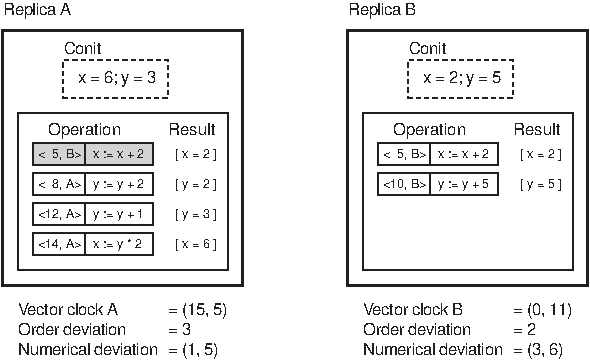
\includegraphics[width=.7\textwidth]{images/07-02}
%
%\begin{block}{Conit: $x$ e $y$ }
%\begin{itemize}
%	\item Relógio vetorial (Vector clock)
%	\item Operação em cinza é permanente
%\end{itemize}
%\end{block}
%\end{frame}
%
%\begin{frame}{Conit}
%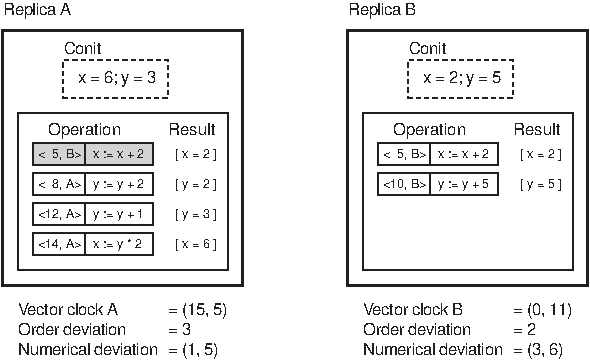
\includegraphics[width=.7\textwidth]{images/07-02}
%
%\begin{block}{Conit: $x$ e $y$ }
%	\begin{itemize}
%		\item A tem três operações não permanentes (pendentes): desvio de ordem = 3.
%		\item B tem duas operações não permanentes: desvio de ordem = 2
%	\end{itemize}
%\end{block}
%\end{frame}
%
%
%\begin{frame}{Conit}
%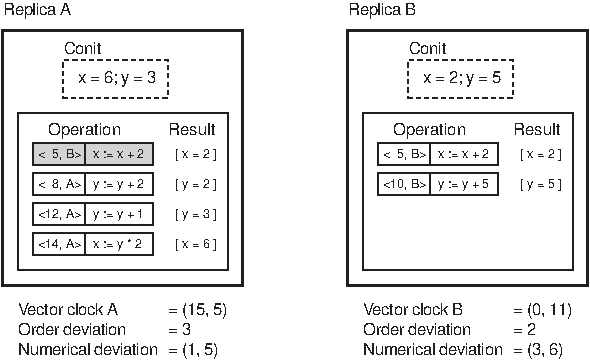
\includegraphics[width=.7\textwidth]{images/07-02}
%
%\begin{block}{Conit: $x$ e $y$ }
%	\begin{itemize}
%		\item A não viu uma operação de B, que muda o valor em 5: desvio numérico (1,5)
%		\item B não viu tês operações de A, que muda o valor em 9: desvio numérico (3,\alert{9})
%	\end{itemize}
%\end{block}
%\end{frame}
%
%
%\begin{frame}{Conit}
%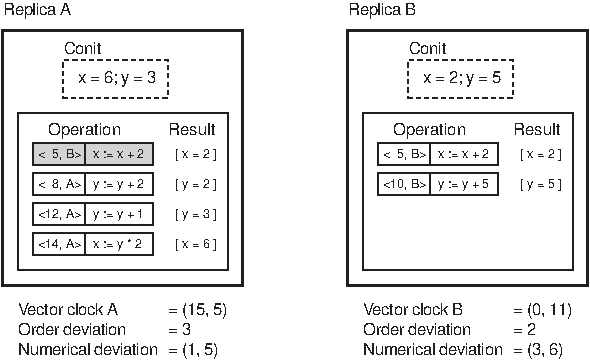
\includegraphics[width=.7\textwidth]{images/07-02}
%
%\begin{block}{Conit: $x$ e $y$ }
%	\begin{itemize}
%		\item A não viu 11 operações de B
%		\item B não viu 15 operações de A
%	\end{itemize}
%\end{block}
%\end{frame}
%
%\begin{frame}{Conit}
%Como manter distância numérica limitada?
%\end{frame}
%

\begin{frame}{Operações Simples}
Modelos desenvolvidos para processamento paralelo, especificando a ordem de execução de operações em múltiplos threads/processos.
\end{frame}


\begin{frame}{Grupos de Operações}
\begin{block}{Ideia}
Efeito de um grupo de operações se torna visível a outros processos ao mesmo tempo. 
Efeitos de operações individuais em um grupo não são visíveis.
\end{block}

\begin{itemize}
	\item Variáveis de sincronização
	\begin{itemize}
		\item Acesso às variáveis de sincronização da datastore é sequencialmente consistente.
		\item Acesso à variável de sincronização não é permitido até que todas as escritas das anteriores tenham sido executadas em todos os lugares.
		\item Acesso aos dados não é permitido até que todas as variáveis de sincronização tenham sido liberadas.
	\end{itemize}
\end{itemize}

\end{frame}

\begin{frame}{Variáveis de sincronização}
\includegraphics[width=.7\textwidth]{images/weaka}

\includegraphics[width=.7\textwidth]{images/weakb}

Materializando variáveis de sincronização na forma de \emph{locks}
\end{frame}


\begin{frame}{Consistência de Entrada}
\begin{itemize}
	\item Lock de leitura só retorna quando todas as mudanças guardadas por aquele lock tiverem sido executadas no processo.
	\item Lock de escrita só retorna quando nenhum outro processo tiver um lock, de leitura ou escrita.
	\item Para ler uma variável, processo deve primeiro contactar o dono atual do lock cercando a variável, para pegar as mais recentes atualizações.
\end{itemize}

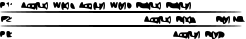
\includegraphics[width=1\textwidth]{images/07-10}
\end{frame}

\begin{frame}{Transações}
Tornam o trancamento/destrancamento de variáveis transparente.
\end{frame}




\subsection{Modelos Centrados nos Clientes}

\begin{frame}{Modelos Centrados nos Clientes}
\begin{block}{Ideia}
	Evitar sincronização global focando-se no que os clientes vêem do sistema. Se para os clientes parecer consistente, tudo bem.
\end{block}

\begin{itemize}
	\item Consistência Eventual
	\begin{itemize}
		\item Se nenhuma escrita ocorrer em período considerável de tempo, os clientes gradualmente se sincronizarão e ficarão consistentes.
		\item Se clientes sempre acessarem as mesmas réplicas, terão impressão de consistência.
	\end{itemize}
	\item Garantias são do ponto de vista de \alert{um} cliente.
	\begin{itemize}
		\item Leituras monotônicas
		\item Escrita monotônicas
		\item Leia suas escritas
		\item Escritas seguem leituras.
	\end{itemize}
\end{itemize}
\end{frame}

\begin{frame}{Modelo de Sistema}
\includegraphics[width=1\textwidth]{images/07-11}

Cliente pode se mover antes de sua última operação ter replicado do servidor onde estava para o novo servidor.
\end{frame}

\begin{frame}[allowframebreaks]{Leituras Monotônicas}
\begin{block}{Garantia}
	Se um processo lê o valor de um item $x$, qualquer leitura sucessiva de $x$ retornará o mesmo valor ou um mais recente.
\end{block}
\begin{itemize}
	\item Toda vez que se conecta a um servidor de email, seu cliente lê novas mensagens, caso haja.
	\item O cliente nunca esquece uma mensagem, mesmo que ainda não esteja no servidor conectado por último.
\end{itemize}

\framebreak

\begin{itemize}
	\item WS($x_i$) -- operações de escrita (\emph{write set}) que levaram a variável $x$ a ter o valor $x_i$.
	\item WS($x_i;x_j$) -- operações de escrita relativas a $x_j$ incluem operações de escrita relativas a $x_i$
\end{itemize}

\includegraphics[width=.5\textwidth]{images/07-12}

\end{frame}


\begin{frame}{Escritas Monotônicas}
\begin{block}{Garantia}
	Se um processo escreve em item $x$, então esta operação deve terminar antes que qualquer escrita sucessiva em $x$ possa ser executada pelo mesmo processo.
\end{block}
\begin{itemize}
	\item Em um sistema de arquivos na rede, a escrita do conteúdo de um arquivo, em certa posição, só pode ser feita se escritas anteriores já estão registradas no arquivo, independentemente de o cliente contactar novo servidor de arquivos.
\end{itemize}


\includegraphics[width=.5\textwidth]{images/07-13}

\end{frame}



\begin{frame}{Leia suas Escritas}
\begin{block}{Garantia}
	Se um processo escreve em item $x$, então leituras sucessivas no mesmo item pelo mesmo processo devem refletir tal escrita.
\end{block}
\begin{itemize}
	\item Atualizar código fonte de uma página e exigir que o navegador carrega a nova versão.
\end{itemize}


\includegraphics[width=.5\textwidth]{images/07-14}

\end{frame}


\begin{frame}{Escritas seguem Leituras}
\begin{block}{Garantia}
	Se um processo lê um item $x$, então escritas sucessivas no mesmo item só podem ser completadas se o mesmo reflete o valor lido anteriormente.
\end{block}
\begin{itemize}
	\item Só é permitido enviar uma resposta a uma mensagem se a mensagem em si é vista, independentemente do cliente ter se movimentado.
\end{itemize}

\includegraphics[width=.5\textwidth]{images/07-15}
\end{frame}



\section{Posicionamento de Réplicas}
\begin{frame}{Posicionamento de Réplicas}
Onde colocar réplicas para conseguir melhor escalabilidade do sistema? Menor custo de comunicação?
\end{frame}

\begin{frame}{Posicionamento de Réplicas}
\begin{itemize}
	\item Objetos (código/dados)
	\item Permanente
	\item Sob demanda do servidor -- por exemplo em uma CDN
	\item Sob demanda do cliente -- por exemplo um cache.
\end{itemize}

\includegraphics[width=\textwidth]{images/07-17}
\end{frame}



\begin{frame}{Sob demanda do Servidor}
\begin{itemize}
	\item $Q$ conta acessos ao arquivo $F$
	\item Agrega acessos por possível réplica mais próxima ($P$)
	\item Número de acessos acima de limiar $R$, replica para $P$
	\item Número de acessos abaixo de $D$, apaga de $P$
	\item $D < R$
	\item Se não é alto o suficiente para replicar nem baixo o suficiente para ignorar (entre $D$ e $R$), considera migrar.
\end{itemize}

\includegraphics[width=.5\textwidth]{images/07-18}
\end{frame}



\begin{frame}{Propagação de Atualizações}
Réplicas precisam ser atualizadas.\pause
\begin{itemize}
	\item Propagar dados -- não reexecuta operações.
	\item Propagar operações -- não copia todos os dados modificados.
	\pause
	\item Propagar notificações -- réplica precisa solicitar atualização.\\ Usado em caches.
\end{itemize}

Melhor opção depende do custo das operações, dados manipulados, e taxa de leitura/escrita dos dados.
\end{frame}

\begin{frame}{Propagação de Atualizações}
Réplicas precisam ser atualizadas.
\begin{itemize}
	\item Propagar dados
	\begin{itemize}
		\item razão leitura/escrita é grande.
		\item operações são caras.
	\end{itemize}
	\item Propagar operações
	\begin{itemize}
		\item razão leitura/escrita é grande.
		\item operações são baratas.
	\end{itemize}
	\item Propagar notificações
	\begin{itemize}
		\item razão leitura/escrita é pequena.
		\item pouco uso da rede
	\end{itemize}
\end{itemize}
\end{frame}



\begin{frame}{Proativo/Push ou Reativo/Pull}
\begin{itemize}
	\item Proativo
	\begin{itemize}
		\item Mantém réplicas consistentes
		\item Desnecessário se leitura $<<$ escrita.
	\end{itemize}
	\item Reativo
	\begin{itemize}
		\item Réplicas só se tornam consistentes quando necessário.
		\item Lento se leitura $>>$ escrita
	\end{itemize}
\end{itemize}

Qual é melhor?
\end{frame}


\begin{frame}{Híbrido: Lease}
\begin{itemize}
	\item Réplica se registra para receber atualizações/notificações por um período.
	\item Estado sobre réplicas é mantido enquanto possível, pelo período contratado.
	\item Em caso de sobrecarga, deixa de mandar atualizações/notificações.
	\item Em caso de lease antigo não renovado, deixa de mandar atualizações/notificações.
	\item Em caso de renovações frequentes, aumenta o período do lease.
\end{itemize}
\end{frame}


